\documentclass{article}
\usepackage[utf8]{inputenc}
\usepackage{graphicx,amsmath,amsfonts,amssymb}

\begin{document}
\title{SVVR Assignment 1}
\author{Sander Nugteren (6042023) \and Merel de Groot (6103677)}
\renewcommand{\today}{November 3, 2014}
\maketitle

\section{Data types}
For this assignment a dataset of cars has to be visualized. The data consists
of the following variables:\\\\
\begin{tabular}{|l|l|}
	\hline
	Variable & Data type \\
	\hline
	Model & Nominal \\
	Miles per Gallon & Quantity (ratio) \\
	Cylinders & Quantity (ratio) \\
	Horsepower & Quantity (ratio) \\
	Weight & Quantity (ratio) \\
	Year & Quantity (interval) \\
	Origin & Nominal\\
	\hline
\end{tabular}

\section{Visual Attribute Choice}
The most important things to show in the visualization in our opinion are the
quantity data types. Because the value ranges for miles per gallon, horsepower and
weight are the largest of the quantitative data, we opted to use the x-, y- and z-axes for these variables. Since the cylinders can only have six discrete values, we decided to use shapes to distinguish these. 
Next, the origin, as it is a nominal variable, is represented by color and the last quantity left, the year of origin, is displayed by color intensity. Since model is a nominal datatype with a huge range (392 instances), it is difficult to represent. We tried to label the datapoints with the model names at first, but this cluttered up the data too much.

\section{The visualization}

\begin{figure}
	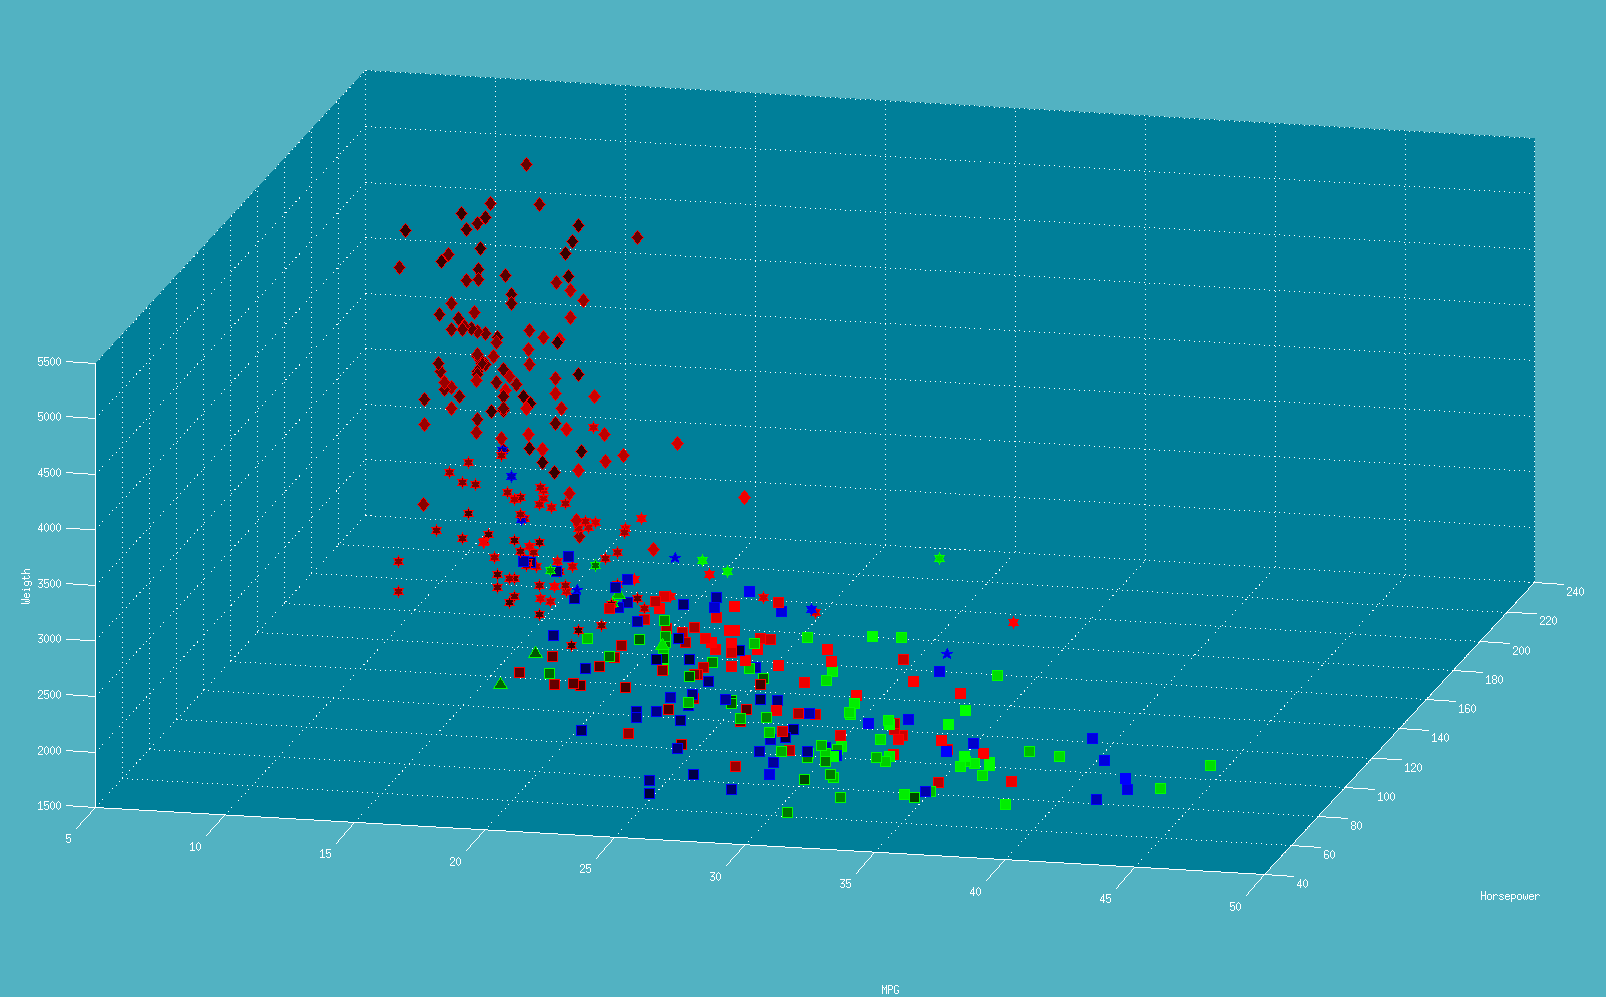
\includegraphics[width=\linewidth]{scivis_plot}
\end{figure}

For the graph we chose a blue background, since this makes the points stand out
more against the background.
We can see many things in this graph. For example, American cars tend to have
lots of cylinders, are heavier and less efficient but have lots of horsepower,
while Japanese cars are lighter and more efficient, but have less horsepower.
Also, the correlation between horsepower and cylinder amount is clearly
visible.

\end{document}
